\documentclass{standalone}
\usepackage{tikz}
\usetikzlibrary{patterns, positioning}
\usepackage[sfdefault]{ClearSans} %% option 'sfdefault' activates Clear Sans as the default text font
\usepackage[T1]{fontenc}

\begin{document}
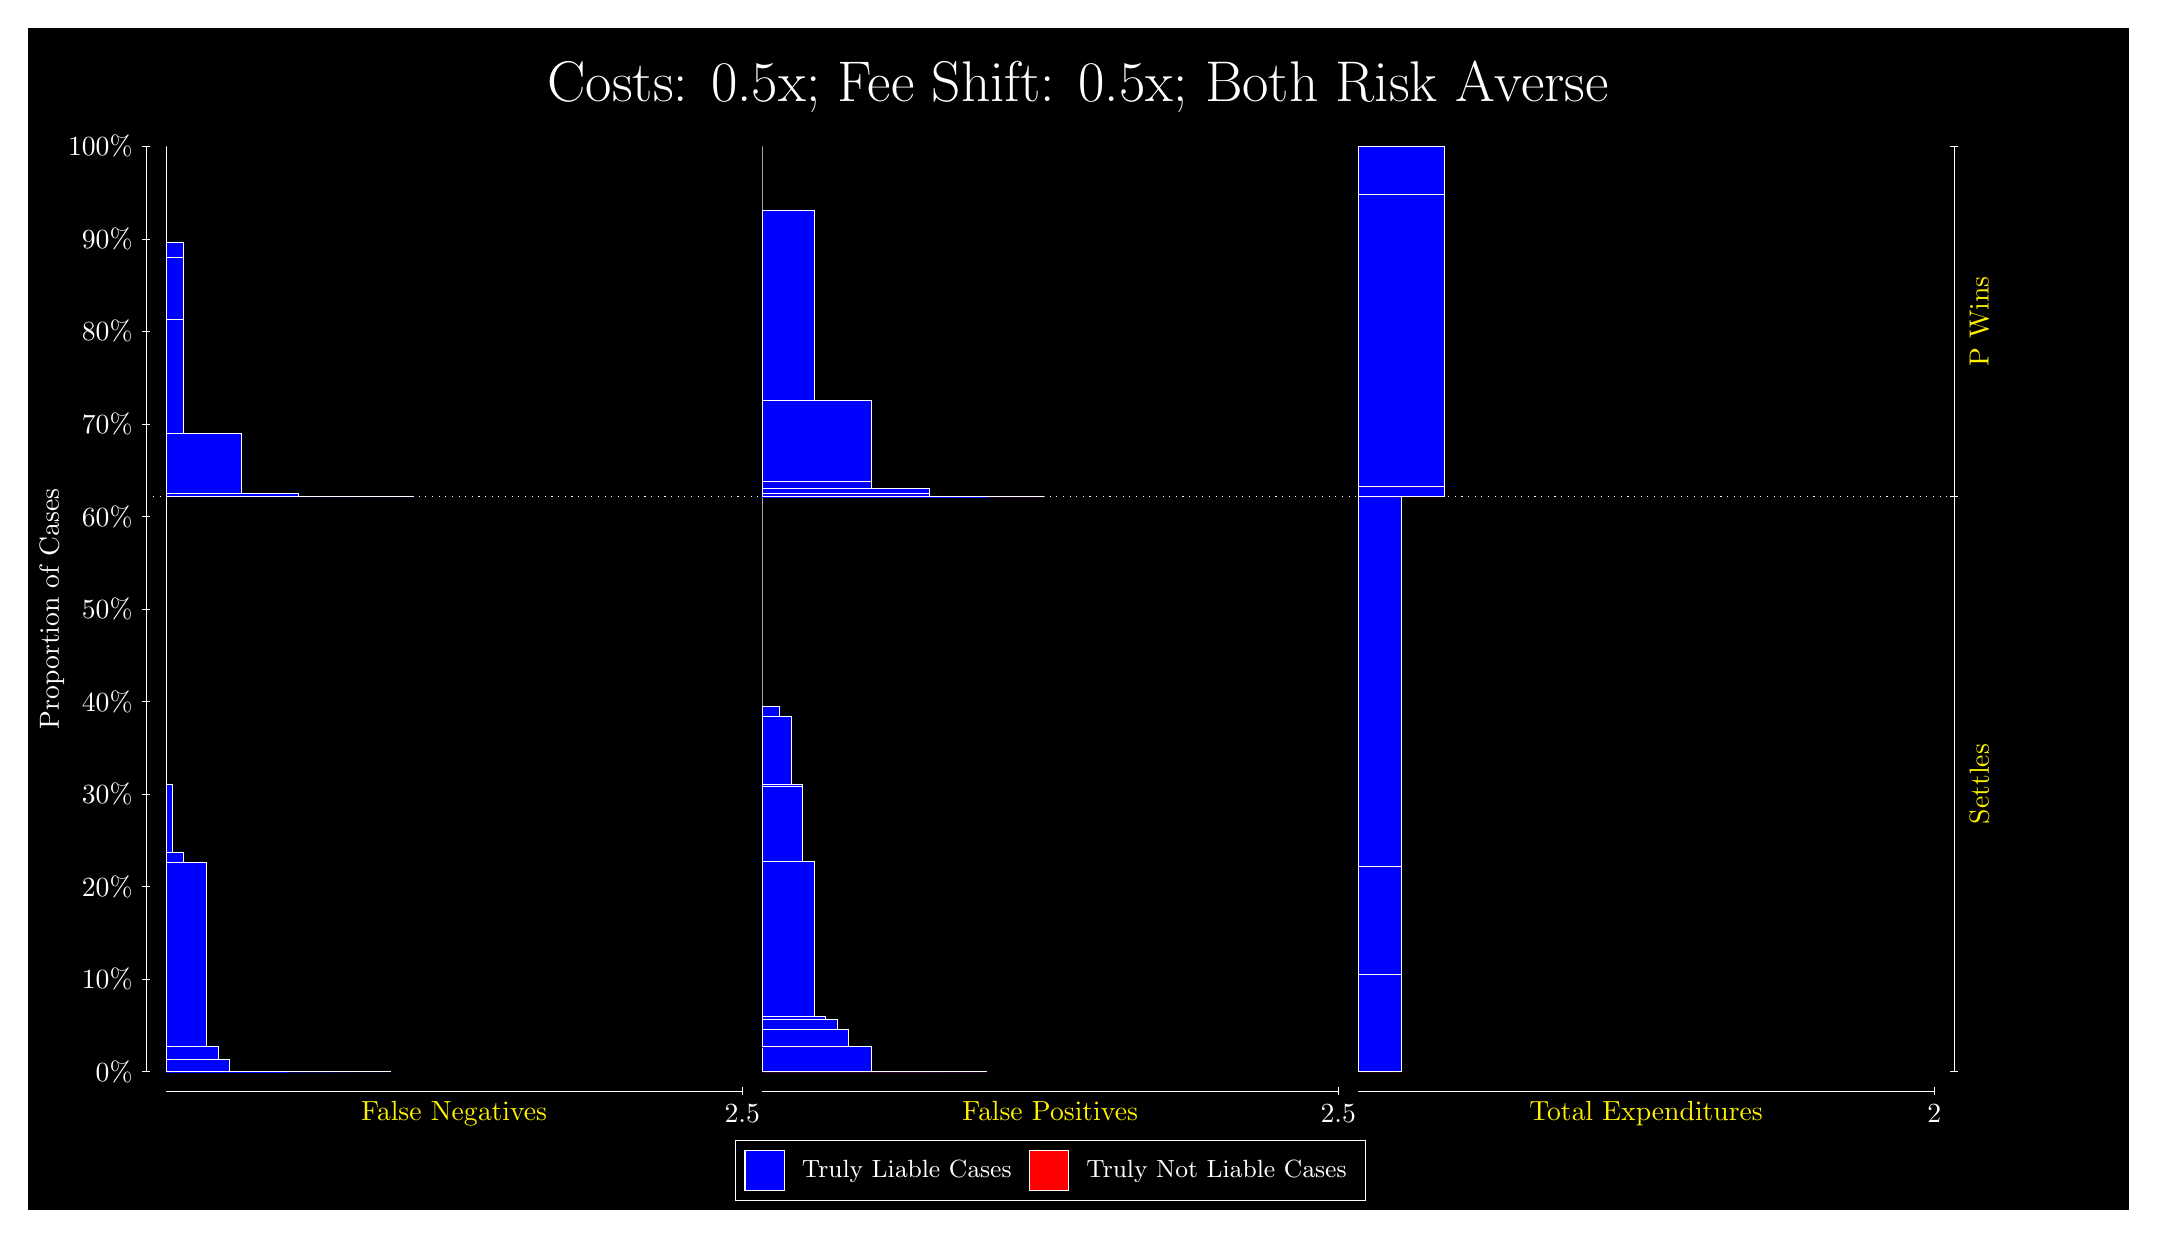
\begin{tikzpicture}
\draw[fill=black] (0,0) rectangle (26.667,15);
\draw[text=white] (0,13.5) rectangle (26.667,15) node[midway] {\huge Costs: 0.5x; Fee Shift: 0.5x; Both Risk Averse};
\draw[white, very thin] (1.5,1.75) -- (1.5,13.5);
\node[rotate=90, text=white, anchor=center] at (0.3, 7.625) {Proportion of Cases};
\draw[white, very thin] (1.45,1.75) -- (1.55,1.75);
\node[text=white, anchor=east] at (1.45, 1.75) {0\%};
\draw[white, very thin] (1.45,2.925) -- (1.55,2.925);
\node[text=white, anchor=east] at (1.45, 2.925) {10\%};
\draw[white, very thin] (1.45,4.1) -- (1.55,4.1);
\node[text=white, anchor=east] at (1.45, 4.1) {20\%};
\draw[white, very thin] (1.45,5.275) -- (1.55,5.275);
\node[text=white, anchor=east] at (1.45, 5.275) {30\%};
\draw[white, very thin] (1.45,6.45) -- (1.55,6.45);
\node[text=white, anchor=east] at (1.45, 6.45) {40\%};
\draw[white, very thin] (1.45,7.625) -- (1.55,7.625);
\node[text=white, anchor=east] at (1.45, 7.625) {50\%};
\draw[white, very thin] (1.45,8.8) -- (1.55,8.8);
\node[text=white, anchor=east] at (1.45, 8.8) {60\%};
\draw[white, very thin] (1.45,9.975) -- (1.55,9.975);
\node[text=white, anchor=east] at (1.45, 9.975) {70\%};
\draw[white, very thin] (1.45,11.15) -- (1.55,11.15);
\node[text=white, anchor=east] at (1.45, 11.15) {80\%};
\draw[white, very thin] (1.45,12.325) -- (1.55,12.325);
\node[text=white, anchor=east] at (1.45, 12.325) {90\%};
\draw[white, very thin] (1.45,13.5) -- (1.55,13.5);
\node[text=white, anchor=east] at (1.45, 13.5) {100\%};

\draw[white, very thin] (24.457,1.75) -- (24.457,13.5);
\draw[white, very thin] (24.407,1.75) -- (24.507,1.75);
\node[anchor=west] at (24.407, 1.75) {};
\draw[white, very thin] (24.407,9.0512) -- (24.507,9.0512);
\node[anchor=west] at (24.407, 9.0512) {};
\draw[white, very thin] (24.407,13.5) -- (24.507,13.5);
\node[anchor=west] at (24.407, 13.5) {};

\draw[white, very thin, fill=blue] (1.75,1.75) rectangle (4.6044,1.75);
\draw[white, very thin, fill=blue] (1.75,1.75) rectangle (4.0188,1.75);
\draw[white, very thin, fill=blue] (1.75,1.75) rectangle (3.8725,1.75);
\draw[white, very thin, fill=blue] (1.75,1.75) rectangle (3.4333,1.75);
\draw[white, very thin, fill=blue] (1.75,1.75) rectangle (3.287,1.7503);
\draw[white, very thin, fill=blue] (1.75,1.7503) rectangle (3.1406,1.7505);
\draw[white, very thin, fill=blue] (1.75,1.7505) rectangle (2.8478,1.7505);
\draw[white, very thin, fill=blue] (1.75,1.7505) rectangle (2.7015,1.7508);
\draw[white, very thin, fill=blue] (1.75,1.7508) rectangle (2.5551,1.9084);
\draw[white, very thin, fill=blue] (1.75,1.9084) rectangle (2.4087,2.0654);
\draw[white, very thin, fill=blue] (1.75,2.0654) rectangle (2.2623,4.4116);
\draw[white, very thin, fill=blue] (1.75,4.4116) rectangle (2.1159,4.4129);
\draw[white, very thin, fill=blue] (1.75,4.4129) rectangle (1.9696,4.5394);
\draw[white, very thin, fill=blue] (1.75,4.5394) rectangle (1.8232,5.3999);
\draw[white, very thin, fill=red] (1.75,5.3999) rectangle (1.75,5.3999);
\draw[white, very thin, fill=blue] (1.75,5.3999) rectangle (1.75,9.0512);
\draw[white, very thin, fill=blue] (1.75,9.0512) rectangle (4.8971,9.0512);
\draw[white, very thin, fill=blue] (1.75,9.0512) rectangle (4.1652,9.0513);
\draw[white, very thin, fill=blue] (1.75,9.0513) rectangle (3.4333,9.0978);
\draw[white, very thin, fill=blue] (1.75,9.0978) rectangle (2.7015,9.8578);
\draw[white, very thin, fill=blue] (1.75,9.8578) rectangle (2.7015,9.859);
\draw[white, very thin, fill=blue] (1.75,9.859) rectangle (1.9696,11.308);
\draw[white, very thin, fill=blue] (1.75,11.308) rectangle (1.9696,12.086);
\draw[white, very thin, fill=blue] (1.75,12.086) rectangle (1.9696,12.277);
\draw[white, very thin, fill=red] (1.75,12.277) rectangle (1.75,12.277);
\draw[white, very thin, fill=blue] (1.75,12.277) rectangle (1.75,13.5);
\draw[white, very thin, fill=red] (9.3189,1.75) rectangle (12.173,1.75);
\draw[white, very thin, fill=blue] (9.3189,1.75) rectangle (12.173,1.75);
\draw[white, very thin, fill=red] (9.3189,1.75) rectangle (11.588,1.75);
\draw[white, very thin, fill=blue] (9.3189,1.75) rectangle (11.588,1.75);
\draw[white, very thin, fill=blue] (9.3189,1.75) rectangle (11.441,1.7505);
\draw[white, very thin, fill=red] (9.3189,1.7505) rectangle (11.295,1.7505);
\draw[white, very thin, fill=blue] (9.3189,1.7505) rectangle (11.295,1.7505);
\draw[white, very thin, fill=red] (9.3189,1.7505) rectangle (11.002,1.7505);
\draw[white, very thin, fill=blue] (9.3189,1.7505) rectangle (11.002,1.7509);
\draw[white, very thin, fill=blue] (9.3189,1.7509) rectangle (10.856,1.7519);
\draw[white, very thin, fill=blue] (9.3189,1.7519) rectangle (10.709,2.0656);
\draw[white, very thin, fill=blue] (9.3189,2.0656) rectangle (10.563,2.067);
\draw[white, very thin, fill=red] (9.3189,2.067) rectangle (10.417,2.067);
\draw[white, very thin, fill=blue] (9.3189,2.067) rectangle (10.417,2.2897);
\draw[white, very thin, fill=blue] (9.3189,2.2897) rectangle (10.27,2.4165);
\draw[white, very thin, fill=blue] (9.3189,2.4165) rectangle (10.124,2.4458);
\draw[white, very thin, fill=blue] (9.3189,2.4458) rectangle (9.9776,4.4198);
\draw[white, very thin, fill=red] (9.3189,4.4198) rectangle (9.8312,4.4198);
\draw[white, very thin, fill=blue] (9.3189,4.4198) rectangle (9.8312,5.3717);
\draw[white, very thin, fill=blue] (9.3189,5.3717) rectangle (9.8312,5.4013);
\draw[white, very thin, fill=blue] (9.3189,5.4013) rectangle (9.6848,6.2618);
\draw[white, very thin, fill=blue] (9.3189,6.2618) rectangle (9.5384,6.3882);
\draw[white, very thin, fill=blue] (9.3189,6.3882) rectangle (9.3921,6.3896);
\draw[white, very thin, fill=blue] (9.3189,6.3896) rectangle (9.3189,9.0512);
\draw[white, very thin, fill=red] (9.3189,9.0512) rectangle (12.905,9.0512);
\draw[white, very thin, fill=blue] (9.3189,9.0512) rectangle (12.905,9.0512);
\draw[white, very thin, fill=blue] (9.3189,9.0512) rectangle (12.173,9.0517);
\draw[white, very thin, fill=red] (9.3189,9.0517) rectangle (12.173,9.0517);
\draw[white, very thin, fill=blue] (9.3189,9.0517) rectangle (12.173,9.0524);
\draw[white, very thin, fill=blue] (9.3189,9.0524) rectangle (11.441,9.0902);
\draw[white, very thin, fill=red] (9.3189,9.0902) rectangle (11.441,9.0902);
\draw[white, very thin, fill=blue] (9.3189,9.0902) rectangle (11.441,9.1528);
\draw[white, very thin, fill=blue] (9.3189,9.1528) rectangle (10.709,9.2404);
\draw[white, very thin, fill=red] (9.3189,9.2404) rectangle (10.709,9.2404);
\draw[white, very thin, fill=blue] (9.3189,9.2404) rectangle (10.709,10.274);
\draw[white, very thin, fill=blue] (9.3189,10.274) rectangle (9.9776,10.276);
\draw[white, very thin, fill=red] (9.3189,10.276) rectangle (9.9776,10.276);
\draw[white, very thin, fill=blue] (9.3189,10.276) rectangle (9.9776,12.692);
\draw[white, very thin, fill=blue] (9.3189,12.692) rectangle (9.3189,13.5);
\draw[white, very thin, fill=red] (16.888,1.75) rectangle (17.437,1.75);
\draw[white, very thin, fill=blue] (16.888,1.75) rectangle (17.437,2.9911);
\draw[white, very thin, fill=red] (16.888,2.9911) rectangle (17.437,2.9911);
\draw[white, very thin, fill=blue] (16.888,2.9911) rectangle (17.437,4.3528);
\draw[white, very thin, fill=red] (16.888,4.3528) rectangle (17.437,4.3528);
\draw[white, very thin, fill=blue] (16.888,4.3528) rectangle (17.437,9.0512);
\draw[white, very thin, fill=red] (16.888,9.0512) rectangle (17.986,9.0512);
\draw[white, very thin, fill=blue] (16.888,9.0512) rectangle (17.986,9.1797);
\draw[white, very thin, fill=red] (16.888,9.1797) rectangle (17.986,9.1797);
\draw[white, very thin, fill=blue] (16.888,9.1797) rectangle (17.986,12.893);
\draw[white, very thin, fill=red] (16.888,12.893) rectangle (17.986,12.893);
\draw[white, very thin, fill=blue] (16.888,12.893) rectangle (17.986,13.5);
\draw[white, dotted] (1.5,9.0512) -- (24.457,9.0512);
\draw[white, very thin] (1.75,1.5) -- (9.0689,1.5);
\node[text=yellow, anchor=north] at (5.4094, 1.5) {False Negatives};
\draw[white, very thin] (9.0689,1.45) -- (9.0689,1.55);
\node[text=white, anchor=north] at (9.0689, 1.45) {2.5};

\draw[white, very thin] (9.3189,1.5) -- (16.638,1.5);
\node[text=yellow, anchor=north] at (12.978, 1.5) {False Positives};
\draw[white, very thin] (16.638,1.45) -- (16.638,1.55);
\node[text=white, anchor=north] at (16.638, 1.45) {2.5};

\draw[white, very thin] (16.888,1.5) -- (24.207,1.5);
\node[text=yellow, anchor=north] at (20.547, 1.5) {Total Expenditures};
\draw[white, very thin] (24.207,1.45) -- (24.207,1.55);
\node[text=white, anchor=north] at (24.207, 1.45) {2};

\node[text=yellow, centered, rotate=90] at (24.777, 5.4006) {Settles};
\node[text=yellow, centered, rotate=90] at (24.777, 11.276) {P Wins};

\draw (12.978300999999998,1.5) node[draw=none] (baseCoordinate) {};
\begin{scope}[align=center]
        \matrix[scale=0.5, draw=white, below=0.5cm of baseCoordinate, nodes={draw}, column sep=0.1cm]{
            \node[rectangle, draw, minimum width=0.5cm, minimum height=0.5cm, fill=blue] {}; &
            \node[draw=none, font=\small, text=white] (B) {Truly Liable Cases}; &
            \node[rectangle, draw, minimum width=0.5cm, minimum height=0.5cm, fill=red] {}; &
            \node[draw=none, font=\small, text=white] (B) {Truly Not Liable Cases}; \\
            };
\end{scope}

\end{tikzpicture}
\end{document}